\begin{frame}{Chriffres clés de 2023 (enquête SNE 2024)}
    \begin{columns}[T,onlytextwidth]
\column{0.50\linewidth}
\small
\begin{itemize}
        \item 283 millions € de chiffre d’affaires
        \item Le numérique : une offre scolaire et universitaire
        \item La littérature en progression (mais seulement 6\% de la production numérique)
        \item L’édition numérique = 10\% du chiffre d’affaires total des éditeurs
    \end{itemize}
\column{0.50\linewidth}
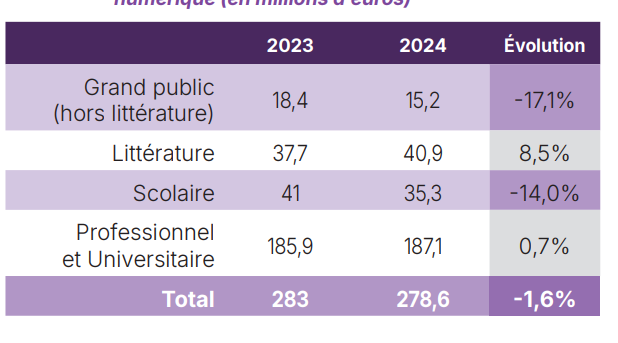
\includegraphics[width=.90\columnwidth]{Images/2024-SNE-numerique.png}
\end{columns}
\end{frame}

\begin{frame}{Chriffres clés de 2023 (enquête SNE 2024)}
    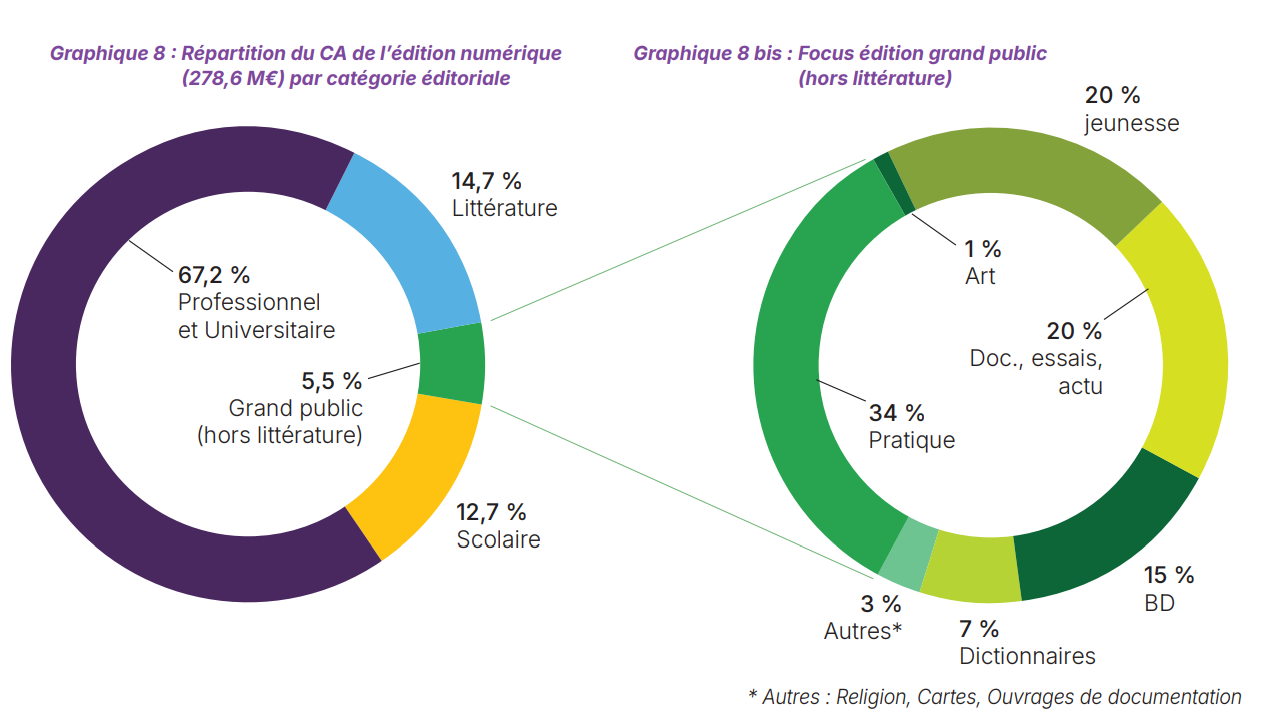
\includegraphics[width=\textwidth]{Images/chiffres-edition-numerique-24.png}
\end{frame}

\begin{frame}{Quelques freins au développement du livre numérique
}
    Plusieurs raisons:
    \begin{itemize}
        \item Économiques: coût de développement trop important; 
        \item Techniques: multiplicité et éparpillement technologique;
        \item Expérimentales: des projets (passionnants), mais peu industrialisés
        \item Médiatiques: l'édition littéraire n'est pas encore conquise par le support numérique.
    \end{itemize}
\end{frame}

\begin{frame}{Les multiples réalités de l'édition numérique}
    \begin{itemize}
        \item Une production homothétique grand public devenue complémentaire à l'offre papier, mais peu intéressante au plan du design éditorial (version Kindle, Koobo des grands titres)
        \item Une production expérimentale relevant de la production de "beau-livre" ou de la micro-édition (éditions indépendantes, auto-édition, cricuits courts)
        \item Des créations éditoriales multi-support, qui relèvent d'une hybridation médiatique (applications numériques, webdoc, fictions transmédiatiques)
    \end{itemize}
\end{frame}